\documentclass[12pt]{article}

\usepackage{sbc-template}
\usepackage{graphicx}
\usepackage{url}
\usepackage[utf8]{inputenc}
\usepackage[T1]{fontenc}
\usepackage[english, portuguese]{babel}
\usepackage{hyphenat}
\hyphenation{mate-mática recu-perar}
\usepackage{amsmath}
\usepackage{graphicx}
\graphicspath{ {imagens/} }
\usepackage{float}
\usepackage{environ}
\usepackage{graphicx}
\usepackage{subfigure}
\usepackage{booktabs}
\usepackage{multirow}

\NewEnviron{myequation}{%
\begin{equation}
\scalebox{1.5}{$\BODY$}
\end{equation}
}

\sloppy

\begin{document} 

\title{Avaliando a Influência da Modelagem Relacional e Colunar no Gerenciamento de Ambientes OLAP por meio do TPC-H}
\author{}
\address{}

\maketitle

\begin{abstract}

Due to data volume growth and companies needs for efficient decision making, 
chosing the best DBMS to Data Warehouse management has been a challenge. Although 
traditional DBMS are yet applied to this purpose, NoSQL approach has emerged 
as an alternative. To evaluate which is the most appropriate, this research 
shows a comparative study between PostgreSQL and MonetDB, through TPC-H benchmark. 
While PostgreSQL achieved good results in a normalized environment, 
MonetDB excelled in general performance.

% Companies have been using data warehouse environments and OLAP applications 
% as decision making support. Due to data volume growth, more efficient ways to 
% process them are needed. Relational DBMS are still widely used, however the NoSQL 
% approach has been consolidating in market. To evaluate which one is the more appropriate 
% in DW management, a comparative study between PostgreSQL and MonetDB DBMS is presented 
% using TPC-H benchmark, under different database sizes. MonetDB was better among 
% denormalized models and PostgreSQL at normalized ones. In general, MonetDB performed 
% better than PostgreSQL.

\end{abstract}
     
\begin{resumo}

Em razão do crescimento do volume de dados 
e da necessidade de agilidade na tomada de decisão das empresas, 
escolher o SGBD mais adequado para o gerenciamento de um 
Data Warehouse tem sido um desafio. Embora os SGBD 
tradicionais ainda sejam utilizados para esse fim, a 
abordagem NoSQL tem surgido como alternativa. 
Para avaliar qual é a mais adequada, este trabalho apresenta 
um estudo comparativo entre os SGBD PostgreSQL e o MonetDB, 
realizado por meio do benchmark TPC-H. Embora o PostgreSQL tenha 
se destacado num ambiente normalizado, o MonetDB apresentou um 
desempenho geral superior.

% Empresas têm utilizado ambientes de data warehouse 
% e aplicações OLAP como apoio à tomada de decisão. 
% Devido ao crescimento do volume de dados, meios mais eficientes para o seu processamento 
% são necessários. SGBD relacionais ainda são bastante utilizados para tal, 
% porém a abordagem NoSQL também vêm se consolidando no mercado. 
% Para avaliar qual é o mais apropriado no gerenciamento de DW, um estudo comparativo entre 
% os SGBD PostgreSQL e o NoSQL MonetDB é aqui apresentado a 
% partir do benchmark TPC-H, com diferentes volumes de dados. O MonetDB se 
% destacou em modelagens mais denormalizadas e o PostgreSQL em modelagens normalizadas; e de maneira geral, 
% o MonetDB obteve desempenho superior ao PostgreSQL.    
\end{resumo}

\section{Introdução}
% Para tomar decisões de maneira rápida as organizações utilizam seus repositórios de dados.
% Conforme o volume destes dados aumenta, a má estruturação do repositório pode degradar o desempenho do acesso às informações,
% e devido a isso a tecnologia de Data Warehouses (DW) é utilizada para persistência de dados e tomada de decisões. 
% Além do armazenamento, é necessário uma aplicação que recupere informações
% de maneira tão eficiente quanto à estruturação do repositório. Aplicações OLAP (\textit{Online Analytical Processing}) 
% analisam dados multidimensionalmente 
% e executam consultas analíticas, fazendo com que estejam fortemente associadas à DW.

\textit{Data Warehouses} (DW) são utilizados para gerenciar 
o armazenamento dos dados de um ambiente de tomada de decisões, 
haja vista o aumento do volume de dados degradar o desempenho do 
acesso às informações em casos onde não há um gerenciador adequado. 
Além do armazenamento, aplicações OLAP (\textit{Online Analytical 
Processing}) 
são utilizadas para recuperar e processar, eficientemente, esses dados, 
tal que estejam fortemente associadas 
ao DW.

Sistemas Gerenciadores de Bancos de Dados (SGBD) surgem como uma solução 
para esta questão, e duas classes de SGBD podem atuar como gerenciadores de DW, os relacionais e os NoSQL. 
Para avaliar a melhor abordagem, a aplicação de um \textit{benchmark} torna-se pertinente, 
e um \textit{benchmark} que se destaca por tratar de sistemas de suporte à decisão é o TPC-H \cite{tpch2017page}. 

Além do SGBD, outro fator que interfere no desempenho de um ambiente OLAP é a forma como este é modelado. 
Ambientes normalizados são utilizados pela facilidade de manutenção,
e o fácil entendimento acerca do relacionamento entre as entidades, o que traz uma visão mais clara do sistema. 
Entretanto, modelos denormalizados surgem para trazer ganho no desempenho das consultas, por diminuir 
as junções entre tabelas devido ao menor número de entidades.

Dadas estas condições, o objetivo aqui é realizar um estudo comparativo entre SGBD relacional e NoSQL 
como gerenciadores de DW utilizando o TPC-H. Devido a seu amplo uso e poucas modificações na linguagem SQL, foi definido o PostgreSQL 
como SGBD relacional e o MonetDB como NoSQL, por este também utilizar SQL, possuir interface simples e ser pioneiro 
entre os NoSQL colunares.

\section{Recuperação e Persistência de Dados}

Um DW é definido como uma coleção de dados não-volátil, orientado ao assunto da organização, 
integrado e variante no tempo \cite{inmon2005building}. É necessário que uma aplicação processe os dados 
contidos no DW e execute consultas analíticas para acessar 
um número massivo de registros, visando informações que dêem suporte à tomada de decisão. Devido a isso, histórico, 
taxa de vazão de consultas e o tempo de resposta são fatores importantes ao processar os dados de um DW.

Aplicações OLAP objetivam identificar tendências, 
padrões de comportamento e anomalias, e ainda relações entre dados \cite{codd1998providing} sob um grande 
volume de dados. Suas consultas são longas, consomem grande tempo de execução e estão interessadas em 
atributos específicos; e o processo de inserção de dados segue um processo conhecido como ETL (extração, transformação e carga), 
sendo mais complexo que pequenas transações \cite{vertabelo2017olap}. É neste processo que a modelagem conceitual do ambiente é definida, 
que tem como base a modelagem dimensional, ou multidimensional, fazendo uma analogia com um cubo para 
a representação de dados, uma vez que uma informação pode ser vista por \textit{n} dimensões. 
Em sua concepção, a modelagem dimensional é composta por tabelas fato e tabelas dimensão.

Fatos representam regras ou métricas de negócio, e geralmente são descritos como atributos 
numéricos, relacionados a quantidades; ou aditivos, pois uma aplicação nunca irá retornar somente um fato, 
mas sim vários onde a operação mais recorrente é a soma de atributos.
Atributos textuais não definem um fato, e na maioria das vezes apenas descrevem algo e são inseridos 
nas tabelas dimensão, que contem descrições a fim de tornar os fatos mais claros. Não é incomum encontrar tabelas dimensão  
com mais de 100 atributos e poucas tuplas, pois a intenção das dimensões é descrever as regras definidas por um 
fato. Nestas entidades são filtradas as consultas, compreendendo agrupamentos, padrões e ordenações, por exemplo.

Modelos dimensionais no escopo de um DW possuem apenas um fato com várias dimensões, fazendo com que 
sua estrutura se assemelhe a uma estrela, sendo conhecidos como modelos estrelas (\textit{star}). Este modelo é 
simples e torna eficiente a recuperação de dados por ter um número menor de junções. Entretanto, com a afirmação de 
que modelos normalizados são mais fáceis para manutenção, em alguns modelos \textit{star} podem ser criadas 
novas tabelas denominadas subdimensão. Estes modelos caracterizam modelagens relacionais, e são conhecidos 
como modelos \textit{snowflake}.

Para comparar o desempenho entre modelagens pode-se utilizar SGBD como gerenciadores de DW, 
com vantagens como controle de redundância, restrições de acesso, 
inserção de índices, restrições de integridade, possibilidade de realizar \textit{backup} e restauração de dados, e persistência 
de dados garantida. Um modelo de SGBD muito conhecido e utilizado é o relacional. Esta classe está atrelada a dados 
normalizados, fazendo com que se aproxime do modelo \textit{snowflake} de DW, 
e preza pelos conceitos de ACID (Atomicidade, Consistência, Isolamento e Durabilidade). Modelos 
assim definidos possuem, porém, algumas limitações quanto à escalabilidade, complexidade e o fato de todas as informações serem 
mantidas e recuperadas sob a forma de tuplas \cite{leavitt2010will}. Tais limitações podem degradar o desempenho de 
um ambiente analítico. 

Para suprir estes problemas SGBD NoSQL podem ser utilizados. Criados com o objetivo de satisfazer algumas deficiências 
de SGBD relacionais, trabalham com modelagens de dados mais denormalizadas e são classificados 
de diferentes formas de acordo com sua estruturação. NoSQL tendem a optar por disponibilidade e particionamento 
de acordo com o teorema CAP (Consistência, Disponibilidade e Partição) \cite{brewer2000towards} 
para realizar operações de forma mais rápida e permitir escalabilidade. 
Uma classe de NoSQL que suporta linguagem SQL é o modelo colunar, cujo 
diferencial é o armazenamento de todas as instâncias de um mesmo atributo junto, e reduz o tempo de acesso e 
escrita em disco \cite{matei2010column, abadi2008query}, retornando apenas os atributos solicitados; e também 
torna possível a compressão de dados \cite{abadi2006integrating} e a eficiência em operações 
matemáticas de agregação \cite{matei2010column}.

\section{TPC-H}
O TPC-H é um \textit{benchmark} de suporte à decisão de negócios, representando grandes volumes de dados e executando 
consultas com um alto grau de complexidade a fim de responder questões críticas de negócio. Ele propõe 
uma modelagem \textit{snowflake} que pode ser encontrada no manual do TPC-H \cite{tpc2017specs}.

O TPC-H não apresenta uma modelagem denormalizada de dados similar à \textit{star}. Para tanto, foi construído 
um ambiente denormalizado a partir do ambiente original do TPC-H para as devidas comparações. 
Essa construção se fundamentou na criação de um modelo com 
uma única entidade fato central, unindo atributos de diferentes fatos, descrita por dimensões, e 
na remoção de tabelas subdimensão.

Em cada modelagem foi executado o teste de desempenho, que é composto de duas execuções: 
o teste de força e o teste de vazão, representados pelas métricas \textit{Power@Size} e \textit{Throughput@Size}, 
onde \textit{Size} representa o tamanho da base de dados. Estas duas execuções são utilizadas para calcular o 
desempenho, que utiliza a unidade de medida \textit{QphH@Size}, que é a quantidade 
de consultas executada por hora para determinado tamanho de banco de dados.

O teste de força mede a taxa de consultas por hora do sistema com um único usuário ativo. 
Neste teste são executadas em uma única sessão três instruções: inserção de novos registros, consultas 
em SQL para recuperar informações, e remoção da mesma quantia de registros inseridos, nesta ordem. O 
segundo teste, o teste de vazão, mede a capacidade de processar a maior quantidade de consultas no menor 
intervalo de tempo simulando vários usuários ativos de maneira concorrente, 
e seu valor é definido pela razão do número total de consultas executadas pelo 
tempo total da execução do teste. 

\section{A Avaliação Experimental}

O estudo foi feito para bases de dados de diferentes tamanhos, estes de 1GB, 10GB e 30GB, a fim de 
verificar o comportamento dos SGBD conforme o volume de dados. Previamente foi analisado 
também o tempo para realizar a carga de dados, notando-se que uma base de dados 
denormalizada leva mais tempo para o carregamento devido à redundância de dados de alguns atributos que 
antes eram tratados em entidades separadas, aumentando o tamanho das entidades das quais eles agora fazem parte. 
Como mostra a Tabela \ref{tab:carregamento}, o MonetDB teve desempenho melhor que o PostgreSQL. 

\begin{table}[htpb]
    \centering
    \caption{Tempo de carregamento em segundos para os cenários de \textit{benchmark}}
    \label{tab:carregamento}
    \begin{tabular}{c|ccc|c}
    \hline
    \multirow{2}{*}{SGBD} & \multicolumn{3}{c|}{Base de Dados (Gb)} & \multirow{2}{*}{Ambiente}  \\
                          & 1           & 10          & 30          &                            \\ \hline
    MonetDB               & 44          & 409         & 1351        & \multirow{2}{*}{\textit{Snowflake}} \\
    PostgreSQL            & 104         & 816         & 4979        &                            \\ \hline
    MonetDB               & 88          & 689         & 2216        & \multirow{2}{*}{\textit{Star}}      \\
    PostgreSQL            & 166         & 2365        & 7216        &                            \\ \hline
    \end{tabular}
\end{table}

Outra variável analisada foi o tamanho final de cada SGBD. A Tabela \ref{tab:carregamento_size} 
mostra que mesmo para a mesma quantidade de dados o MonetDB tem o tamanho em bytes reduzido, e um 
fator que explica isso é a capacidade que um SGBD colunar tem de realizar compressão 
de dados de forma mais eficiente.

\begin{table}[htpb]
    \centering
    \caption{Tamanho do banco de dados em Mb para os cenários de \textit{benchmark}}
    \label{tab:carregamento_size}
    \begin{tabular}{c|ccc|c}
        \hline
        \multirow{2}{*}{SGBD} & \multicolumn{3}{c|}{Base de Dados (Gb)} & \multirow{2}{*}{Ambiente}  \\
                              & 1           & 10          & 30          &                            \\ \hline
        MonetDB               & 771         & 8087        & 21352       & \multirow{2}{*}{\textit{Snowflake}} \\
        PostgreSQL            & 1567        & 15510       & 44371       &                            \\ \hline
        MonetDB               & 952         & 9352        & 26271       & \multirow{2}{*}{\textit{Star}}      \\
        PostgreSQL            & 2565        & 25487       & 71586       &                            \\ \hline
        \end{tabular}
    \end{table}

O processo do TPC-H foi desenvolvido utilizando o \textit{driver JDBC}, 
cada qual disponível na página oficial dos SGBD, devido à simplificação 
que seu uso traz ao desenvolvimento de aplicações, e por dar suporte a diferentes SGBD. 
Os resultados dos testes de força e vazão para o ambiente normalizado 
podem ser observados na Tabela \ref{tab:power-vazao-normalizado}. 
No MonetDB o teste de força 
mostrou-se superior para todas as bases de dados, porém o teste de vazão 
apresenta comportamento diferente conforme a carga de dados aumenta, evidenciando um desempenho 
melhor do PostgreSQL em relação ao MonetDB.

\begin{table}[htpb]
    \centering
    \caption{Valores dos testes de força e vazão para os cenários normalizados}
    \label{tab:power-vazao-normalizado}
    \begin{tabular}{c|ccc|c}
    \hline
    \multirow{2}{*}{SGBD} & \multicolumn{3}{c|}{Base de Dados (Gb)} & \multirow{2}{*}{Execução}        \\
                      & 1            & 10          & 30         &                                  \\ \hline
    MonetDB               & 14043.395    & 11861.997   & 5457.325   & \multirow{2}{*}{Power@Size}      \\
    PostgreSQL            & 1222.570    & 870.994    & 363.441    &                                  \\ \hline
    MonetDB               & 1622.929     & 330.479     & 112.572    & \multirow{2}{*}{Throughput@Size} \\
    PostgreSQL            & 958.028      & 364.541     & 220.005    &                                  \\ \hline
    \end{tabular}
\end{table}

Ao contrário do cenário normalizado, no denormalizado o MonetDB obteve valores 
superiores ao PostgreSQL em ambos os testes. A Tabela \ref{tab:power-vazao-denormalizado} 
evidencia que o MonetDB em ambiente denormalizado consegue ter ganhos 
em relação ao normalizado para cenários com mais de um usuário ativo.

\begin{table}[htpb]
    \centering
    \caption{Valores dos testes de força e vazão para os cenários denormalizados}
    \label{tab:power-vazao-denormalizado}
    \begin{tabular}{c|ccc|c}
    \hline
    \multirow{2}{*}{SGBD} & \multicolumn{3}{c|}{Base de Dados (Gb)} & \multirow{2}{*}{Execução}        \\
                      & 1            & 10          & 30         &                                  \\ \hline
    MonetDB               & 21811.705    & 17902.155   & 6873.122   & \multirow{2}{*}{Power@Size}      \\
    PostgreSQL            & 659.758    & 190.307    & 149.514    &                                  \\ \hline
    MonetDB               & 2468.02      & 583.560     & 165.419    & \multirow{2}{*}{Throughput@Size} \\
    PostgreSQL            & 637.310      & 149.455     & 120.578    &                                  \\ \hline
    \end{tabular}
    \end{table}

Os valores de execução dos testes de força e vazão foram aplicados 
no cálculo de desempenho final para o \textit{benchmarking}. Ao avaliar de forma isolada,  
o MonetDB destacou-se na modelagem \textit{star} por ser mais denormalizada, com 
ganhos de 54\%, 63\% e 36\%.  
O PostgreSQL, por ser relacional, teve perdas de 40\%, 70\% e 53\% 
no ambiente \textit{star} em relação ao \textit{snowflake}. 
As Figuras \ref{fig:qph_monet} e \ref{fig:qph_psql} ilustram os resultados 
em conjunto de seus valores para o MonetDB e o PostgreSQL, respectivamente. 

\begin{figure*}[htpb]
    \centering
    \subfigure[]{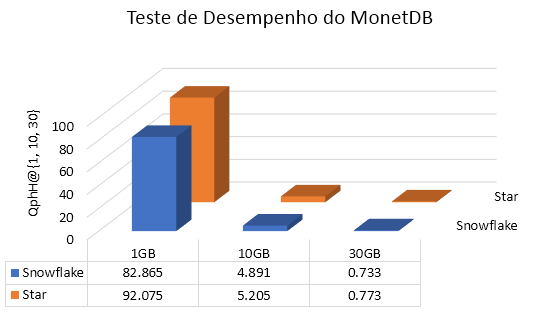
\includegraphics[width=7.2cm]{qph_monetdb}\label{fig:qph_monet}}
    \subfigure[]{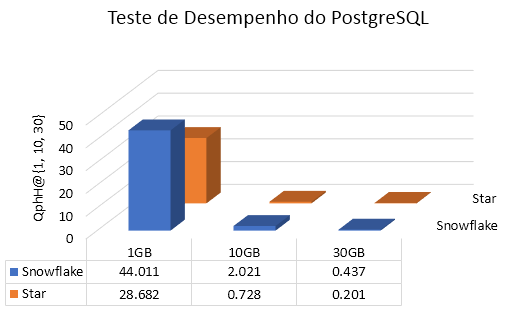
\includegraphics[width=7.2cm]{qph_postgres}\label{fig:qph_psql}}
    \caption{Ilustração dos resultados entre os SGBD}\label{fig:qph_sgbd}
\end{figure*}

\begin{figure*}[htpb]
    \centering
    \subfigure[]{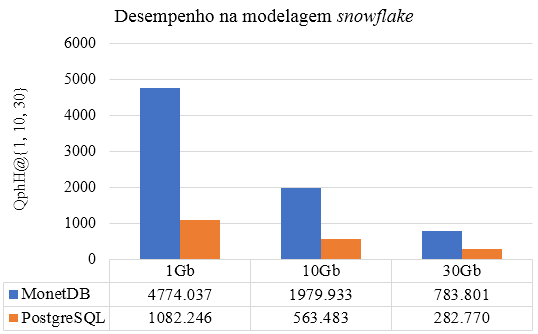
\includegraphics[width=7.2cm]{qph_snowflake}\label{fig:qph_snowflake}}
    \subfigure[]{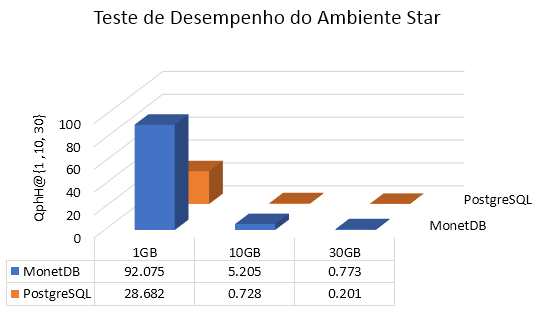
\includegraphics[width=7.2cm]{qph_star}\label{fig:qph_star}}
    \caption{Ilustração dos resultados entre os ambientes}\label{fig:qph_ambiente}
\end{figure*}

Dados os ambientes e comparando os SGBD, o MonetDB obteve ganhos sob o PostgreSQL 
em todos os cenários. Este resultado era esperado se considerado o armazenamento 
e leitura aprimorados do MonetDB, apesar dos resultados apresentados pelo teste de força. 
Os ganhos para as bases de dados foram de 341\%, 251\% e 177\% no ambiente 
normalizado e 1031\%, 1817\% e 694\% no ambiente denormalizado, como ilustrado 
nas Figuras \ref{fig:qph_snowflake} e \ref{fig:qph_star}.

\section{Conclusão e Trabalhos Futuros}

Com todos os ganhos superiores a 100\% e 
com seu melhor valor sendo em torno de dezenove vezes melhor que o do PostgreSQL, 
corrobora-se a ideia de que um SGBD NoSQL pode trazer vantagens para ambientes OLAP 
bases de dados pequenas e grandes; 
tanto à leitura quanto carregamento e armazenamento de dados,  
por adaptar-se melhor à modelagem denormalizada comumente utilizada em DW e 
por realizar compressão de dados. 
Com mais de um usuário ativo o PostgreSQL mostrou que 
atuando sobre uma base de dados normalizada um SGBD relacional pode obter resultados 
melhores que um NoSQL. 

Como continuidade da pesquisa, propõe-se a inclusão de mais SGBD NoSQL de 
diferentes classes para analisar se a mudança na estruturação de SGBD 
que não utilizam SQL para manipulação do banco tem impacto direto em ambientes empresariais. 
Ainda, a aplicação dos resultados do estudo em 
empresas que utilizam uma modelagem relacional juntamente com SGBD relacionais, para 
de verificar se a mudança para um NoSQL sob modelagem denormalizada trará melhorias no desempenho 
de suas aplicações.

\bibliographystyle{sbc}
\bibliography{REFERENCES}

\end{document}
